\chapter{Design}
\label{chapter:Design}
%Overarching design in a top-down view: 
%-server/client design overall architecture, system model
%-describe file system, 
%-how protocol is peformed by the server
%-describe current functionality of the implementation. Handles protocol run, view-changes and checkpointing

%old version:-overall usage over different parameters, overaching stuff thats not the actual implementation of the algorithm, but the network layer to server to algorithm, how to run the algorithm/checkpointing/view changes.
%first draft!!!
This chapter presents an overall summary of our \ac{pbft} application implementation. This includes a description of the system architecture used for the \ac{pbft} network. Additionally, to better understand the workflow of the application, a summary of our code structure is given. Finally, a description is provided for the current application design. Primarily specifying which parts of the program take advantage of the Cleipnir framework and how the server side interacts with the protocol workflow.
%Remember to check previous sections for how I should mark names in the text!
\section{Network Architecture}
\begin{figure}
	\centering
	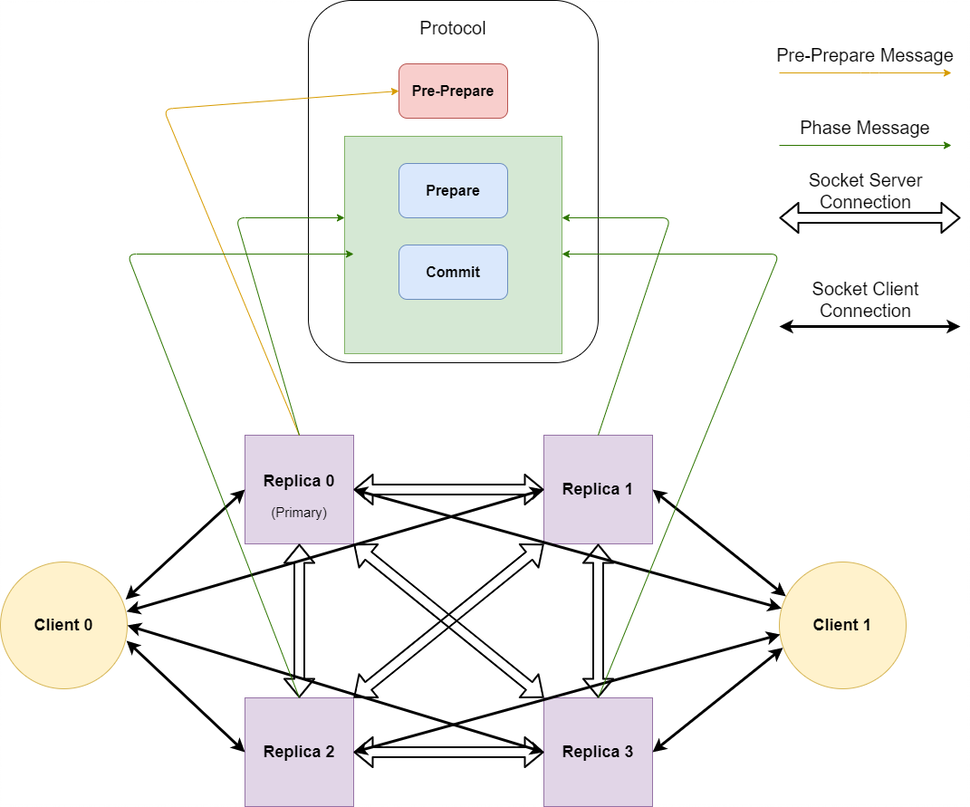
\includegraphics[width=\linewidth]{figures/meshnetwork}
	\caption{Overall architecture of the \ac{pbft} implementation networking}
	\label{fig:meshnetwork}
\end{figure}
%NEED TO REDESIGN SO THAT NETWORK IS MENTION IN ONE PART AND OTHER STUFF IN ANOTHER SUBTITLE
The \autoref{fig:meshnetwork} shows the system architecture used for \ac{pbft} implementation. Generally our network architecture follows the same structure as the system model introduced in \autoref{sec:systemModel}. The system consists of four server implementations called \emph{replicas}, where the replica with the lowest identifier value is chosen as the primary. These four replicas are communicating over a mesh network using socket connections. This means each replica shares a unique network socket with each other replica in the \ac{pbft} network. To avoid creating multiple socket connections between two replicas, the replica with the highest identifier is the one tasked with being the initiator when creating the socket connection. Because of this the primary replica is not required to be an active party when establishing any connections to its fellow replicas. The primary instead establishes all its socket connections by listening for any connection attempts on its local network address. The opposite scenario occurs for the replica with the highest identifier value. Although the replica still listens for connections on its local network address in the case where a higher replica does exist in the network, it is also responsible for initiating the socket connections with all the other replicas in the network that have lower identifier values to its own.

When the replicas have established connections, the replicas can still not fully communicate with each other until they have exchanged public keys. This is required so that messages between replicas can be verified using a digital signature. Public keys are exchanged in \emph{session messages}, which are messages that are automatically sent between replicas once a socket connection has been established. If the public keys are for some reason not exchanged, then the replica discards any message received from that host. If the message received from the unknown host happens to be a \emph{request} or a protocol related message, the replica also terminates the connection. This also applies for clients. This current public key model is unfortunately not very secure. This is due to public keys being ephemeral, therefore it needs to be updated and replaced in the case the replica’s execution is interrupted or stopped. Currently in this implementation, the private and public key pair for a replica are created randomly at system start-up. Currently there is no way for the replicas to authenticate another replica after it has rebooted. A replica must therefore replace the key value pair representing a replica's public key in its register if it receives a new session message with the same replica identifier value. This in turn means the system is susceptible to impersonation and spoofing attacks~\cite{ WEB:spoofingAttack}. Because the main goal of this thesis focuses more on the aspects behind implementing a simple \ac{pbft} workflow, the current cryptographic system was deemed sufficient for simulating a network using digital signatures. However, it is important to be aware of this major security flaw of the system so that it can be potentially fixed in the future. Not to mention avoid similar problems in the future.


\section{Overview of Workflow}
The system performs the \ac{pbft} protocol by exchanging protocol messages over the mesh network until at least three of the servers have finished all three protocol phases. In this implementation protocol messages. The \ac{pbft} protocol is triggered when the server receives a request from one of the connected client nodes. The primary is responsible for officially starting an instance of the \ac{pbft} protocol by multicasting a protocol message of type pre-prepare. There are two important goals for the pre-prepare phase. The first is to make sure that the replicas have an agreement upon the ordering of the request. In other words, the replicas will perform the requests in the same order as the primary, which in turn means the request should have the same sequence numbers throughout the network. The second important goal is to determine whether or not the primary is fit to be leader. As mentioned in section \autoref{sec:view-change}, a view-change occurs when a leader no longer is eligible. In our application the view-changes are triggered by timeout which are set once a replica receives a client's request. If the primary takes too long in the pre-prepare phase, then the timeout will exceed and the other replicas will perform a view-change in order to change the primary replica. Although it would be useful to have timeouts in the commit phase in the instance where the majority of servers are unable to properly finish the commit phase, it is currently not supported in our implementation due to how timeouts are handled inside the protocol workflow(should probably be moved elsewhere). The rest of the replicas will be the responsible party during the prepare phase by sending protocol messages of type prepare, while every replica will participate in the commit phase using commit type protocol messages. The last step of current \ac{pbft} implementation is to create a reply message and send it back to the client responsible for the request. The details in regards to the \ac{pbft} workflow implementation will be discussed in \autoref{chapter:Imp}.

\section{Code structure}
In the figure we \autoref{fig:filestruct} can see a short summary of the code structure for our \ac{pbft} replica. The summary shows folders containing our implementation for necessary items for the \ac{pbft}. The summary also highlights some of the more important files, meaning files that contain the most relevant code segments for the application.

%REWRITE SO THAT THE FOCUS IS ON THE Code structure how protocol functionality is %divided into different class objects and divided etc. Then talk about the server.cs <--> %workflow relationship, started by App.cs

\subsection{Protocol Objects}
To start off, the \ac{pbft} algorithm uses a lot of different types of message for the replicas to collaborate. For simplicity we stored all of the classes revolving messages within the \emph{Message} folder. Since the protocol messages share traits and functionality, we introduced two interfaces to reduce redundancy. The first interface regards the serialization process for transforming the messages into byte streams so that they can be exchanged over the \ac{tcp} network~\cite{WEB:tcp}. The other interface is for the digital signature process. Session messages are not signed, therefore they do not inherit this interface. In addition, to reduce complexity we set the normal workflow protocol messages such as pre-prepare, prepare and commit messages, to use a single class object known as \code{Phase Messages}. View-change and checkpoint messages are instead represented with their own unique class object.

To store the proof of an \ac{pbft} iteration, we implemented class objects known as \emph{certificates} that are found in the \emph{Certificates} folder. The implemented certificate objects essentially have the same functionality as the different certificates described in \autoref{chapter:PBFT} for the \ac{pbft} algorithm. Certificates act as records showing the status of the state of protocol iteration, where a single iteration requires 2 valid certificates in order to finish. Just like the protocol messages, we implement both protocol certificate types by an object class known as \code{Protocol certificate} where the protocol types are determined by a single variable. Checkpoints and view-changes once again have their own class object for their certificate proof. There are also interfaces used to avoid redundant code for the certificate objects.

\subsection{Other functionalities}
The static functionalities that are not tied to any object classes are placed in the \emph{Helper} folder. This includes functionality for serializing and deserializing messages objects with JSON~\cite{WEB:NewJSON}, cryptographic functions related to creating and validating digital signatures and files containing all the enum types used for this implementation. An enum is essentially a predefined dotnet class that has only constant values which are defined upon initialization and is really useful for classifying other objects~\cite{WEB:Enum}. In our \ac{pbft} implementation we have for instance used enums to categorize the protocol phase a phase message belongs to. This allows the program to easily distinguish between pre-prepare, prepare and commit phase messages even when they all use the same object type.

The \emph{JSONFiles} folder contains the JSON files which have information about the network addresses for each of the replicas in the system designated to their receptive identifier values. There exist two JSON files in this folder. The first file is used when running the implementation over multiple systems or over docker containers. The second file uses localhost addresses with different port numbers that are meant to be used when testing the system on a local device.

The \ac{pbft} replica implementation uses Cleipnir to persist important parts of the code in order for servers to easily be able to reconnect to the system. As discussed in \autoref{chapter:Cleipnir}, Cleipnir has several different engine types which can be used to serialize and store the applications data. In our \ac{pbft} replica implementation, we have decided to use the \emph{Simple File Storage} engine. The \emph{Storage} folder will contain the .txt files in which Cleipnir stores its data in. Since there are several instances of replicas in the \ac{pbft} network, the name of the .txt file used to store the application data will follow the structure "PBFTStorage" with the replicas identifier value at the end of the name.

The \emph{Replica} folder contains code which is directly related to the server or code which are directly related to the protocol. The \emph{Replica} folder has two sub folders in order to easier distinguish code based on their functionality. All the networking code that is not directly connected to the server side network handling is placed inside the subfolder \emph{Network}. This includes the code for creating sockets and functions for properly handling the data received from the socket by the TCP network protocol.
The \emph{Protocol} sub folder contains code which is directly related to the protocol execution. This includes code related to the execution of the main workflow of the \ac{pbft} algorithm. In addition, code for handling the reactive execution for view-change and checkpointing are also placed here.
The other files in the \emph{Replica} folder contains code that helps the replica run properly, including code which is used to help communication between server side and protocol workflow run inside Cleipnir.

\subsection{Notable Files}
The \emph{App.cs} file contains the code which starts all the processes needed in the \ac{pbft} replica. This includes code for starting Cleipnir, creating a server instance and starting the protocol handlers. This file also includes the main application state, which in this implementation is simply a list of operations theoretically performed by the system.

The \emph{Server.cs} file is by far the largest. This is due to the server this implementation  acts as the bridge linking the network layer, responsible for sending and receiving messages properly, to the active protocol workflow which requires the result of said messages. In general the server is also responsible for the other server side operations.

The \emph{Workflow.cs} file is where the code for normal protocol workflow and view-change workflow occurs. The \autoref{chapter:Imp} introduces in detail how the workflows are implemented.
%\newpage
\begin{wrapfigure}{r}{0.45\linewidth}
\centering
%\vspace{15pt}
%\rule{0.9\linewidth}{0.75\linewidth}
% ,scale=0.8, every node/.style={scale=0.8}
\tikzstyle{every node}=[draw=black,thick,anchor=west]
    \begin{tikzpicture}[%
      grow via three points={one child at (0.5,-0.7) and
      two children at (0.5,-0.7) and (0.5,-1.4)},
      edge from parent path={(\tikzparentnode.south) |- (\tikzchildnode.west)}]
      \node {PBFT}
        child { node {App.cs}}
        child { node {Certificates}
        	child {node {...}}
        	}	
        child [missing] {}
        child { node {Messages}
        	child {node {...}}
        	}
        child [missing] {}
        child { node {Helper}
        	child {node {...}}
        	}
        child [missing] {}
        child { node {JSONFiles}
        	child {node {serverInfo.json}}
        	child {node {testServerInfo.json}}
        	}
        child [missing] {}
        child [missing] {}
        child { node {Storage}
        	child {node {...}}
        }
        child [missing] {}
        child { node {Replica}
          child { node {Server.cs}}
          child { node {Network}
          	child {node {...}}
        	}
        }
        child [missing] {
          child { node {Protocol}
          child { node {Workflow.cs}}
          child { node {...}}
        	}
        };
\end{tikzpicture}
    \caption{Summary of the file architecture for the PBFT implementation}
    \label{fig:filestruct}
    \vspace{40pt}
\end{wrapfigure}

\begin{figure}[H]
	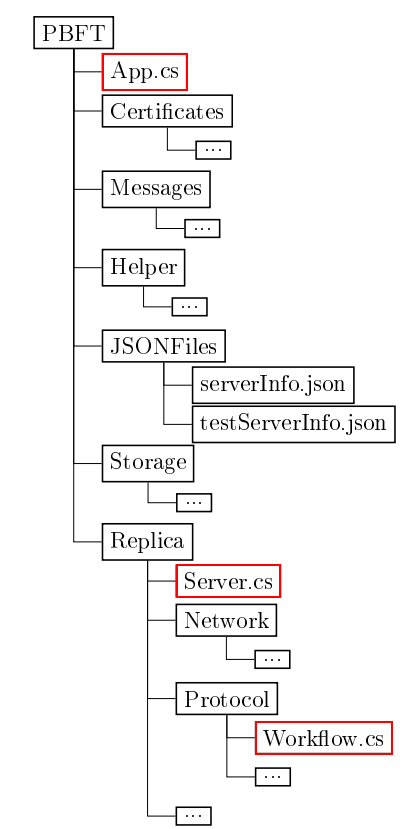
\includegraphics[width=0.45\linewidth]{figures/filestructtest}
	\caption{Summary of the file architecture for the \ac{pbft} implementation}
    \label{fig:filestruct}
\end{figure}

\newpage

\section{Persistent vs Ephemeral}
%This will be a very large part, just need to figure out how to structure it.
%Before we can introduce the main PBFT implementation workflow, it is first important to introduce the relationship between the server side and the protocol workflow. 
\label{sec:persvsephe}
An important detail when using the Cleipnir framework is to have a general idea for which parts of the system are desired to be persistent. As mentioned in \autoref{section:PersistentProgramming}, Cleipnir allows for hybrid persistent programming. Therefore, it is important to know which data is needed to be persisted for the consensus algorithm, so that it can be easily reinstated after a system shutdown. In addition, it is important to avoid storing unnecessary data as it will generally slow down the synchronization period. Another reason as to why making a distinct divide between persistent and ephemeral parts of the code is important is due to the difficulties encountered when using \code{CTask} together with traditional asynchronous operations as mention in \autoref{section:PersistentProgramming}. In our case, because our goal is to evaluate both async/await and Cleipnir for implementation of consensus algorithms, its important to not interchange these tools as it would in most cases lead to race conditions.

\autoref{fig:PersistencyEphemeral} shows parts of our \ac{pbft} implementation being divided into persistent parts and ephemeral parts. In general, static functions and objects unrelated to the \ac{pbft} workflow are treated as ephemeral. Meanwhile objects related to the \ac{pbft} implementations, \code{Source} objects and functions that handles workflow related to the \ac{pbft} protocol are persisted. The server is an exception as some parts are persistent while others parts are not. As an example, the protocol logger is stored in the server and is persisted, on the other hand anything related to networking is not persisted. In a sense the operations occurring in the server are treated as a bridge between the persistent parts as well as the ephemeral parts. By this we mean the server is responsible for handling any messages received from the socket connections. These messages are then emitted to their respective reactive operators which are run in the persistent part and are waiting for changes to occur. There are a few exceptions to this rule, case in point if the message is needed for server-side rather than any \ac{pbft} protocol workflows, the message is instead used directly by the server. A primary example of this being session messages. However, in order for the servers non-persistent network handler to be perform operations which affects the persistent part run by Cleipnir, the operation must be scheduled by Cleipnir's execution engine. There are two reasons for this syntax. Firstly, code run by Cleipnir is not supposed to be affected by code outside of Cleipnir. Similarly to the case where using an asynchronous operations within \code{CTask}, attempting to emit a message or perform an operation which changes the state of a persisted object, will most of the time cause the same scenario we discussed earlier. New threads will occur and Cleipnir will attempt to perform the operation concurrently, however this scenario is not thread safe and sooner or later will affect the state of the system negatively. Secondly, running the operations by the Cleipnir's execution engine attempts to enforce the FCFS approach as mention in \autoref{section:CleipnirOv}. This will in turn make it a lot easier to keep track of the operations as it will give the illusion of synchronously system. The only situation we experienced where the Cleipnir execution engine didn't follow the FCFS scheduling algorithm was then the next operations was stuck, in which the second operation in the queue was executed instead and so forth. \autoref{code:schedulerEmit} shows an example of where the server uses the Cleipnir engine reference to schedule a phase message to be emitted to the \emph{ProtocolSubject} \code{Source} object. To summarize the primary relationship between the server, the network layer and the persistent workflow implementations is simply that the server will emit any messages it receives from the network layer and then emit these messages to the persistent workflows. As it is required for the \ac{pbft} protocol and view-change protocol to multicast messages during their process, these implementations have a direct reference to the server. In order to accomplish this, both persistent workflow shares a common persistent object known as \code{ProtocolExecution}. This means the protocol algorithms can easily send any messages it needs to the server through the server referance in the \code{ProtocolExecution}. 

This design is unfortunately not perfect. Because the server requires to schedule the operations in order for protocol execution to move on with its execution. In some scenarios we've encountered where the scheduled process never finishes its execution. Normally this wouldn't be a problem, however in some cases it is quite a severe problem. Usually when scheduling an operation which requires emitting to a \code{source} object without any receivers, the operation obviously will never finish. Nevertheless, when the server attempts to schedule an additional operations afterwards, the operation is never scheduled, which in turn leads to the application being deadlocked. This situation seems to be similar to sending messages to a channel without any receivers in Golang\cite{WEB:golangChannels}, in spite of that this is an issue which rarely occur, but when it does it is detrimental to the system. Therefore, to counteract this issue, strict conditions are placed in the server to avoid sending messages to reactive subjects in the situations where there are no listeners. %may be too vague.

\begin{figure}[H]
	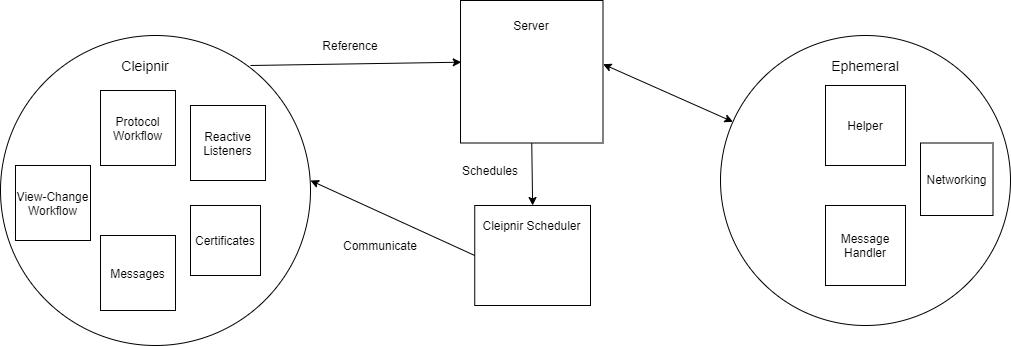
\includegraphics[width=\linewidth]{figures/CleipnirStructure}
	\caption{Application divided into persistent parts and ephermeral parts and how they interact}
	\label{fig:PersistencyEphemeral}
\end{figure}

\begin{figure}[h]
	\centering
	%\lstset{style=sharpc}
	\begin{lstlisting}[label = code:schedulerEmit, caption= Example of server and protocol interaction using Cleipnir scheduler, captionpos=b, basicstyle=\scriptsize]
	public void EmitPhaseMessageLocally(PhaseMessage mes)
        {
            Console.WriteLine("Emitting Phase Locally!");
            if (ProtocolActive)
            {
                _scheduler.Schedule(() =>
                {
                    Subjects.ProtocolSubject.Emit(mes);
                });    
            }
        }
	\end{lstlisting}
\end{figure}